\documentclass[14pt,a4paper]{extarticle}

% Сборка: pdflatex main.tex (два раза для обновления оглавления).
\usepackage[T2A]{fontenc}
\usepackage[utf8]{inputenc}
\usepackage[russian]{babel}
\usepackage[left=30mm,right=15mm,top=20mm,bottom=20mm]{geometry}
\usepackage{amsmath,amssymb}
\usepackage{graphicx}
\usepackage{indentfirst}
\usepackage{setspace}
\usepackage[unicode,hidelinks]{hyperref}
\graphicspath{{./src/}}

\onehalfspacing
\setlength{\parindent}{1.25cm}
\setlength{\parskip}{0pt}
\hypersetup{
    pdfauthor={Нуртдинов Ренат Маратович}
}

\begin{document}

\begin{titlepage}
    \begin{center}
        [УдГУ]\\
        {[Название факультета]}\\
        {[Название кафедры]}

        \vfill

        \textbf{КУРСОВАЯ РАБОТА}\\[0.5cm]
        на тему:\\[0.3cm]
        \textbf{«Кратчайшие пути в графах»}
    \end{center}

    \vspace{2cm}

    \begin{flushright}
        Нуртдинов Ренат Маратович\\[0.5cm]
        Руководитель: [ФИО, должность]
    \end{flushright}

    \vfill

    \begin{center}
        Ижевск --- \the\year
    \end{center}
\end{titlepage}

\tableofcontents
\newpage

\section*{Введение}
\addcontentsline{toc}{section}{Введение}

Задача поиска кратчайших путей является одной из основных задач теории
графов. Она возникает при построении маршрутов в транспортных сетях,
передаче данных в компьютерных сетях и планировании последовательности
действий с минимальными затратами. В таких задачах объекты и связи между
ними представляются в виде графа, а вес каждого ребра характеризует
расстояние, время, стоимость или другую числовую величину. Требуется найти
путь, для которого сумма весов входящих в него рёбер минимальна.

Актуальность темы связана с необходимостью эффективно обрабатывать сети
большого размера, строить маршруты для транспорта и выбирать алгоритм с 
учётом особенностей исходных данных.
Метод решения зависит от того, является ли граф взвешенным, допускаются ли
отрицательные веса рёбер и требуется ли найти путь между двумя вершинами,
расстояния от одной вершины до всех остальных или расстояния между всеми
парами вершин. Поэтому изучение кратчайших путей включает не только описание
алгоритмов, но и анализ условий их применимости и вычислительной сложности.

\textbf{Цель работы} --- изучить основные алгоритмы поиска кратчайших путей
в графах и сравнить их применимость к различным типам задач, проанлизировать
новый алгоритм поиска кратчайшего пути(C-HD) и сравнить его с алгоритмом Дейкстры.

Для достижения поставленной цели необходимо решить следующие задачи:
\begin{enumerate}
    \item Рассмотреть основные понятия теории графов и способы представления
    графов в памяти компьютера.
    \item Сформулировать задачу поиска кратчайшего пути и выделить её
    основные разновидности.
    \item Изучить поиск в ширину, алгоритмы Дейкстры, Беллмана--Форда
    и Флойда--Уоршелла, C-HD.
    \item Сравнить условия применимости алгоритмов, их временную сложность
    и требования к памяти.
    \item Реализовать выбранные алгоритмы и исследовать их работу на
    тестовых графах.
    \item Исследовать выбранные алгоритмы на разных условиях.
\end{enumerate}

\textbf{Объект исследования} --- графы, моделирующие связи между объектами. \\
\textbf{Предмет исследования} --- алгоритмы поиска кратчайших путей,
их свойства и эффективность.

В работе предполагается использовать методы теории графов, анализ
алгоритмов и вычислительный эксперимент. Практическая часть будет включать
проверку корректности реализации на небольших графах с известными ответами
и сравнение времени выполнения на графах различного размера и плотности, сравнение
скорости алгоритмов от колличества используемых ядер процессора.

Работа состоит из введения, трёх разделов, заключения и списка использованных
источников. В первом разделе рассматриваются теоретические основы задачи с точки зрения алгебры,
во втором --- теоритические основы алгоритмов и работы процессора, в третьем --- реализация и сравнение
алгоритмов.

\newpage
\section{Теоретические основы поиска кратчайших путей}

\subsection{Основные понятия теории графов}
% Раскрыть понятия вершины, ребра, ориентированного и неориентированного
% графа, пути, цикла и веса ребра.

Для начала сформулируем основные понятия, которые будут использоваться дальше.
Графом будем называть несколько точек (вершин), некоторые пары которых соединены 
отрезками (рёбрами). Граф связный, если от каждой вершины можно дойти до 
любой другой по этим отрезкам. Циклом назовём какой-то путь по рёбрам графа,
начинающегося и заканчивающегося в одной и той же вершине. И ещё граф 
называется взвешенным, если каждому ребру соответствует какое-то число (вес).
Не может быть двух рёбер, соединяющих одни и те же вершины. \\
Граф обозначается как $G=(V,E)$, где $V$ --- множество вершин,
а \\ $E$ $\subseteq V \times V$ --- множество рёбер . Для взвешенного 
графа задаётся функция весов
$w\colon E\to\mathbb{R}$. Вес пути $P$, состоящего из рёбер
$e_1,e_2,\ldots,e_k$, определяется суммой
\[
    L(P)=\sum_{i=1}^{k}w(e_i).
\] \\
Далее при описании сложности алгоритмов будут использвоваться следующие 
обозначаения: \\
$ | n | $ --- колличество вершин \\
$ | m | $ --- колличество ребер \\
В невзвешенном графе длиной пути считается число его рёбер.

\subsection{Постановка задачи}
Для заданных вершин $s$ и $t$ необходимо найти путь из $s$ в $t$
минимального веса. Если вершина $t$ недостижима из $s$, расстояние
принимается равным $+\infty$. Задача при отрицальном цикле из $s$ не будет
рассматрниваться т.к. в таком случае, можно бесконечно уменьшать кратчайшее
расстояние.

\subsection{Способы представления графов}
Графы можно представить различными способами, в том числе с
помощью матрицы смежности, списков смежности и списка рёбер.
Например граф на рисунке 1 является ориентированным графом без веса на ребрках
\\

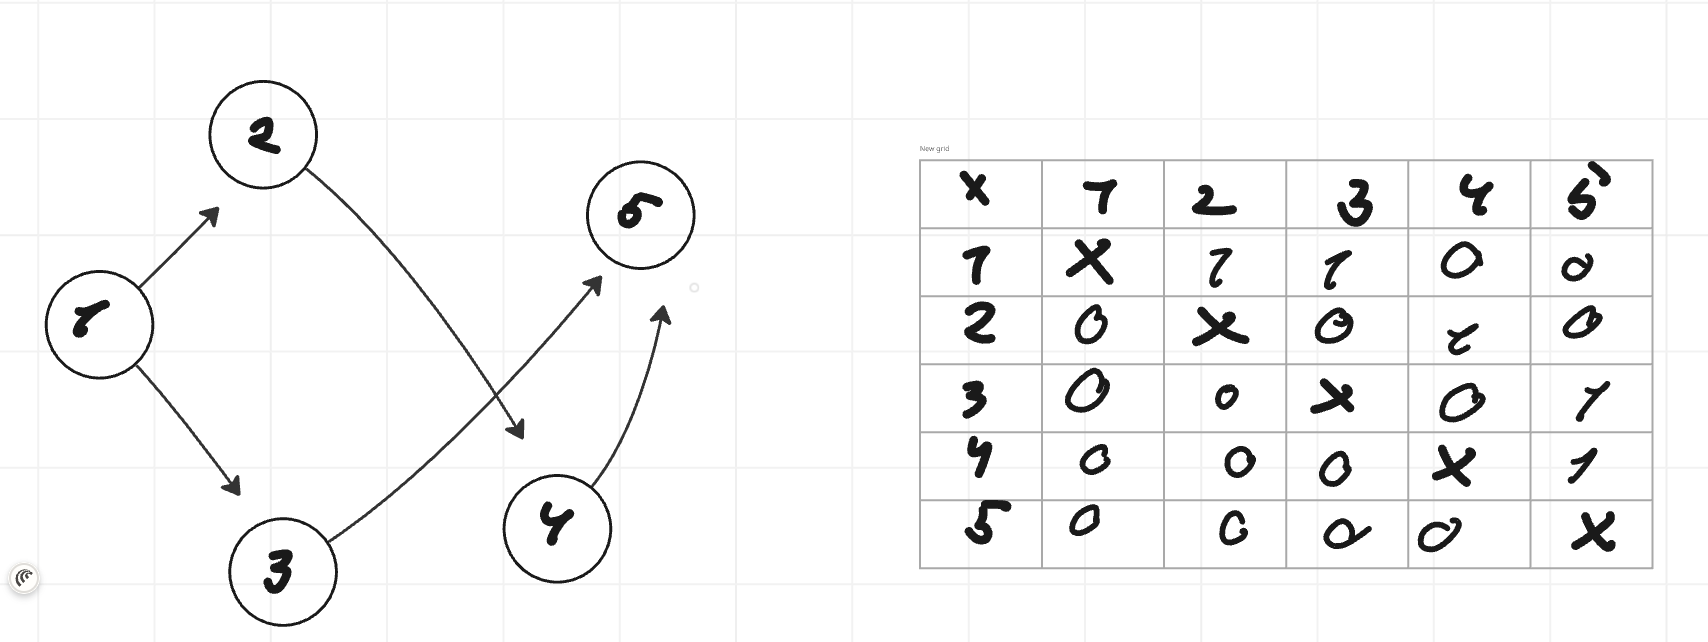
\includegraphics[width=6in]{1graph_without_weight.png}

В данном примере граф представлен с помощью списка смежности, где каждая 
вершина содержит 1 если она соеденена с другой вершиной и 0 если не соединена. \\
На данном примере n = 5, m = 6. \\
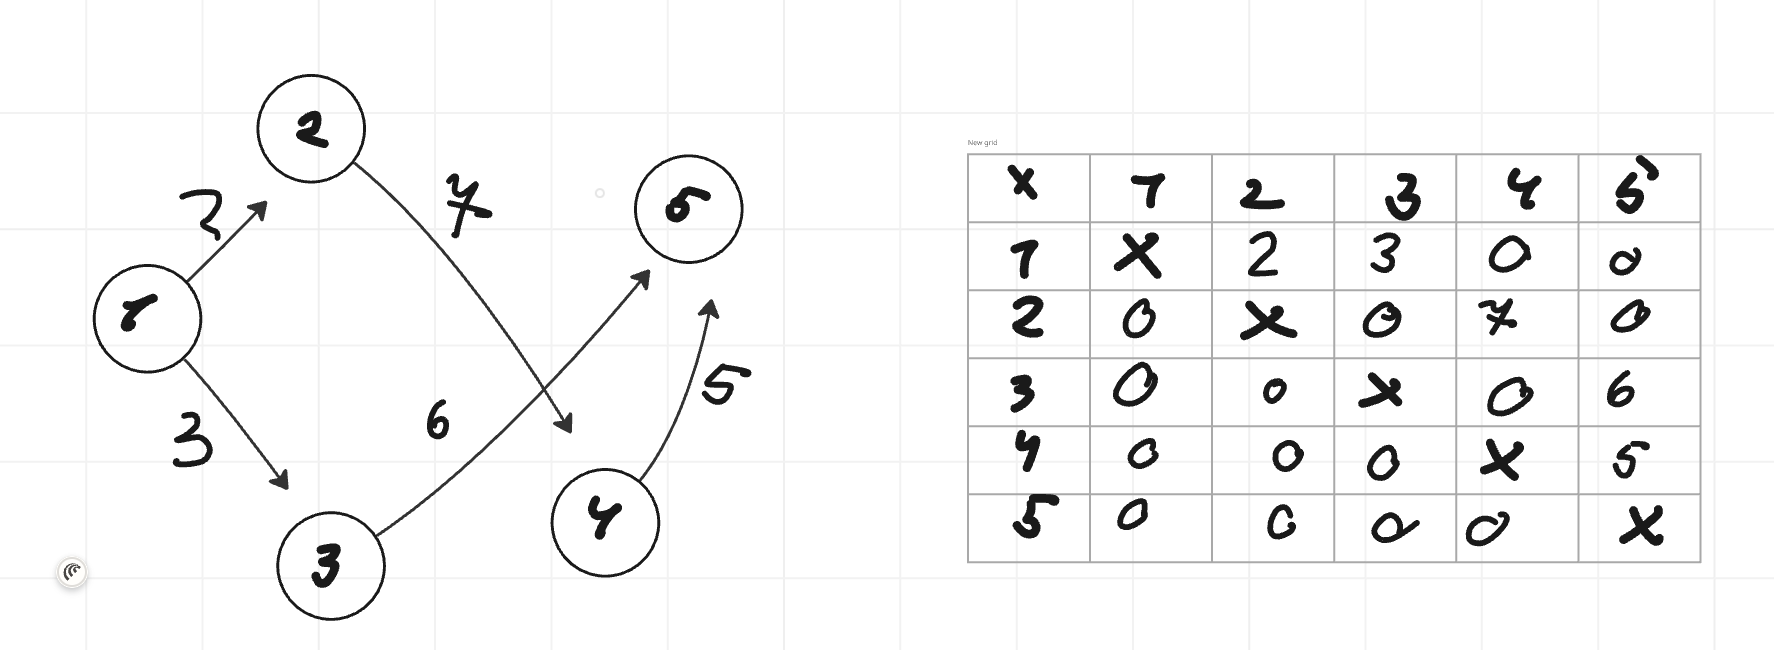
\includegraphics[width=6in]{2graph_with_weight.png} \\
На рисунке 2 представлен ориентированный граф с весами на рёбрах. В
данном примере граф представлен с помощью списка смежности, где каждая 
вершина содержит вес пути если она соеденена с другой вершиной и 0 если
не соединена.

\newpage

\section{устройство работы процессора}

\subsection{как работают ядра процессора}
В компьютере может быть несколько ядер процессора, которые могут выполнять
разные задачи одновременно. Каждому ядру подается набор команд, которое
оно выполняет. Так же ядра могут обмениваться данными между собой, что позволяет
ускорить выполнние задач. Но переодически ядра могут не выполнять никакие
команды т.к. для выполнения задачи требуется информация, которая находится в
другом ядре. В таком случае ядро будет простаивать, пока не получит необходимую
информацию. 
\section{Алгоритмы поиска кратчайших путей}

\subsection{Поиск в ширину}
% Рассмотреть кратчайшие пути в невзвешенном графе, очередь и сложность
% O(|V| + |E|) при использовании списков смежности.


\subsection{Алгоритм Беллмана--Форда}
% Описать повторные релаксации и обнаружение достижимых отрицательных циклов.

\subsection{Алгоритм Флойда--Уоршелла}
% Привести динамическое соотношение для расстояний между всеми парами вершин.


\subsection{Алгоритм Дейкстры}
% Описать релаксацию, выбор ближайшей вершины и очередь с приоритетом.
% Указать требование неотрицательности весов рёбер.

\subsection{Алгоритм C-HD}

\subsection{Принцип работы процессора}


\subsection{Сравнение алгоритмов}
% Добавить таблицу: задача, ограничения на веса, время работы, память.
% Для каждой оценки сложности указать используемые структуры данных.

\newpage
\section{Практическая реализация и исследование}

\subsection{Описание реализации}
% Указать язык программирования, формат входных данных и способ
% восстановления пути по найденным расстояниям или предкам вершин.

\subsection{Тестирование корректности}
% Рассмотреть связные и несвязные графы, нулевые веса, несколько
% кратчайших путей, отрицательные рёбра и отрицательные циклы.
% Подбирать тесты с учётом ограничений каждого алгоритма.

\subsection{Результаты экспериментов}
% Описать генерацию графов, условия измерений и число повторов.
% Добавить реальные результаты, таблицы и графики после экспериментов.

\newpage
\section*{Заключение}
\addcontentsline{toc}{section}{Заключение}
% После выполнения работы сформулировать результаты по каждой задаче
% из введения и рекомендации по выбору алгоритма.

\newpage
\section*{Список использованных источников}
стаатьи: \\
\href{https://habr.com/ru/articles/957702/}{Разбираемся с Р и Е (habr)}
\addcontentsline{toc}{section}{Список использованных источников}
% Добавить фактически использованные книги, статьи и документацию.
% Оформить ссылки в соответствии с требованиями учебного заведения.

\end{document}
